\documentclass[a4paper,12pt]{article}

% don't forget the document class, generally : \documentclass[a4paper,12pt]{article}

\usepackage[utf8]{inputenc}
\usepackage[french]{babel}
\usepackage{graphicx}
\usepackage{gensymb}
\usepackage{amsmath}
\usepackage{float}
\usepackage{scrextend}
\usepackage{caption} 
\usepackage{siunitx}
\usepackage{enumitem}
\usepackage{amsthm}
\usepackage{fancyhdr}
\usepackage{amssymb}
\usepackage{wrapfig}
\usepackage{geometry}
\usepackage{standalone}
\usepackage{import}
\usepackage[usenames, dvipsnames]{color}

 \usepackage{biblatex} % manages bibliography and references
\addbibresource{sample.bib}


\geometry{hmargin=1in, vmargin=1in}

 \newenvironment{absolutelynopagebreak}
 {\par\nobreak\vfil\penalty0\vfilneg
 \vtop\bgroup}
 {\par\xdef\tpd{\the\prevdepth}\egroup
 \prevdepth=\tpd}
 
 \pagestyle{fancy}                        
\fancyhf{}                               
\fancyhf[HL]{Application des maths}                
\fancyhf[HR]{Géométrie euclidienne}             
\fancyhf[FC]{\thepage/\pageref{Lastpage}}
 
\newtheorem{definition}{Définition}[section]
\newtheorem{theorem}{Théorème}
\newtheorem{corollary}{Corollaire}[theorem]
\newtheorem{lemma}[theorem]{Lemme}
\newtheorem*{hyp}{Hypothèse}
\newtheorem*{concl}{Conclusion}
\newtheorem*{remark}{Remarque}

\captionsetup{format=default,labelformat=simple,labelsep=colon,
justification=justified,font={sf,small},labelfont=bf,
textfont=default} 



\begin{document}

\pagebreak
\subsection{Théorème des diagonales du parallélogramme}
\begin{theorem}\label{th:parallelogramme}
Les diagonales d'un parallélogramme se coupent en leur milieu.
\end{theorem}

\begin{proof}
Nous considérons un parallélogramme $ABCD$ dont les diagonales se coupent au point $O$.

\begin{figure}[H]
        \centering
        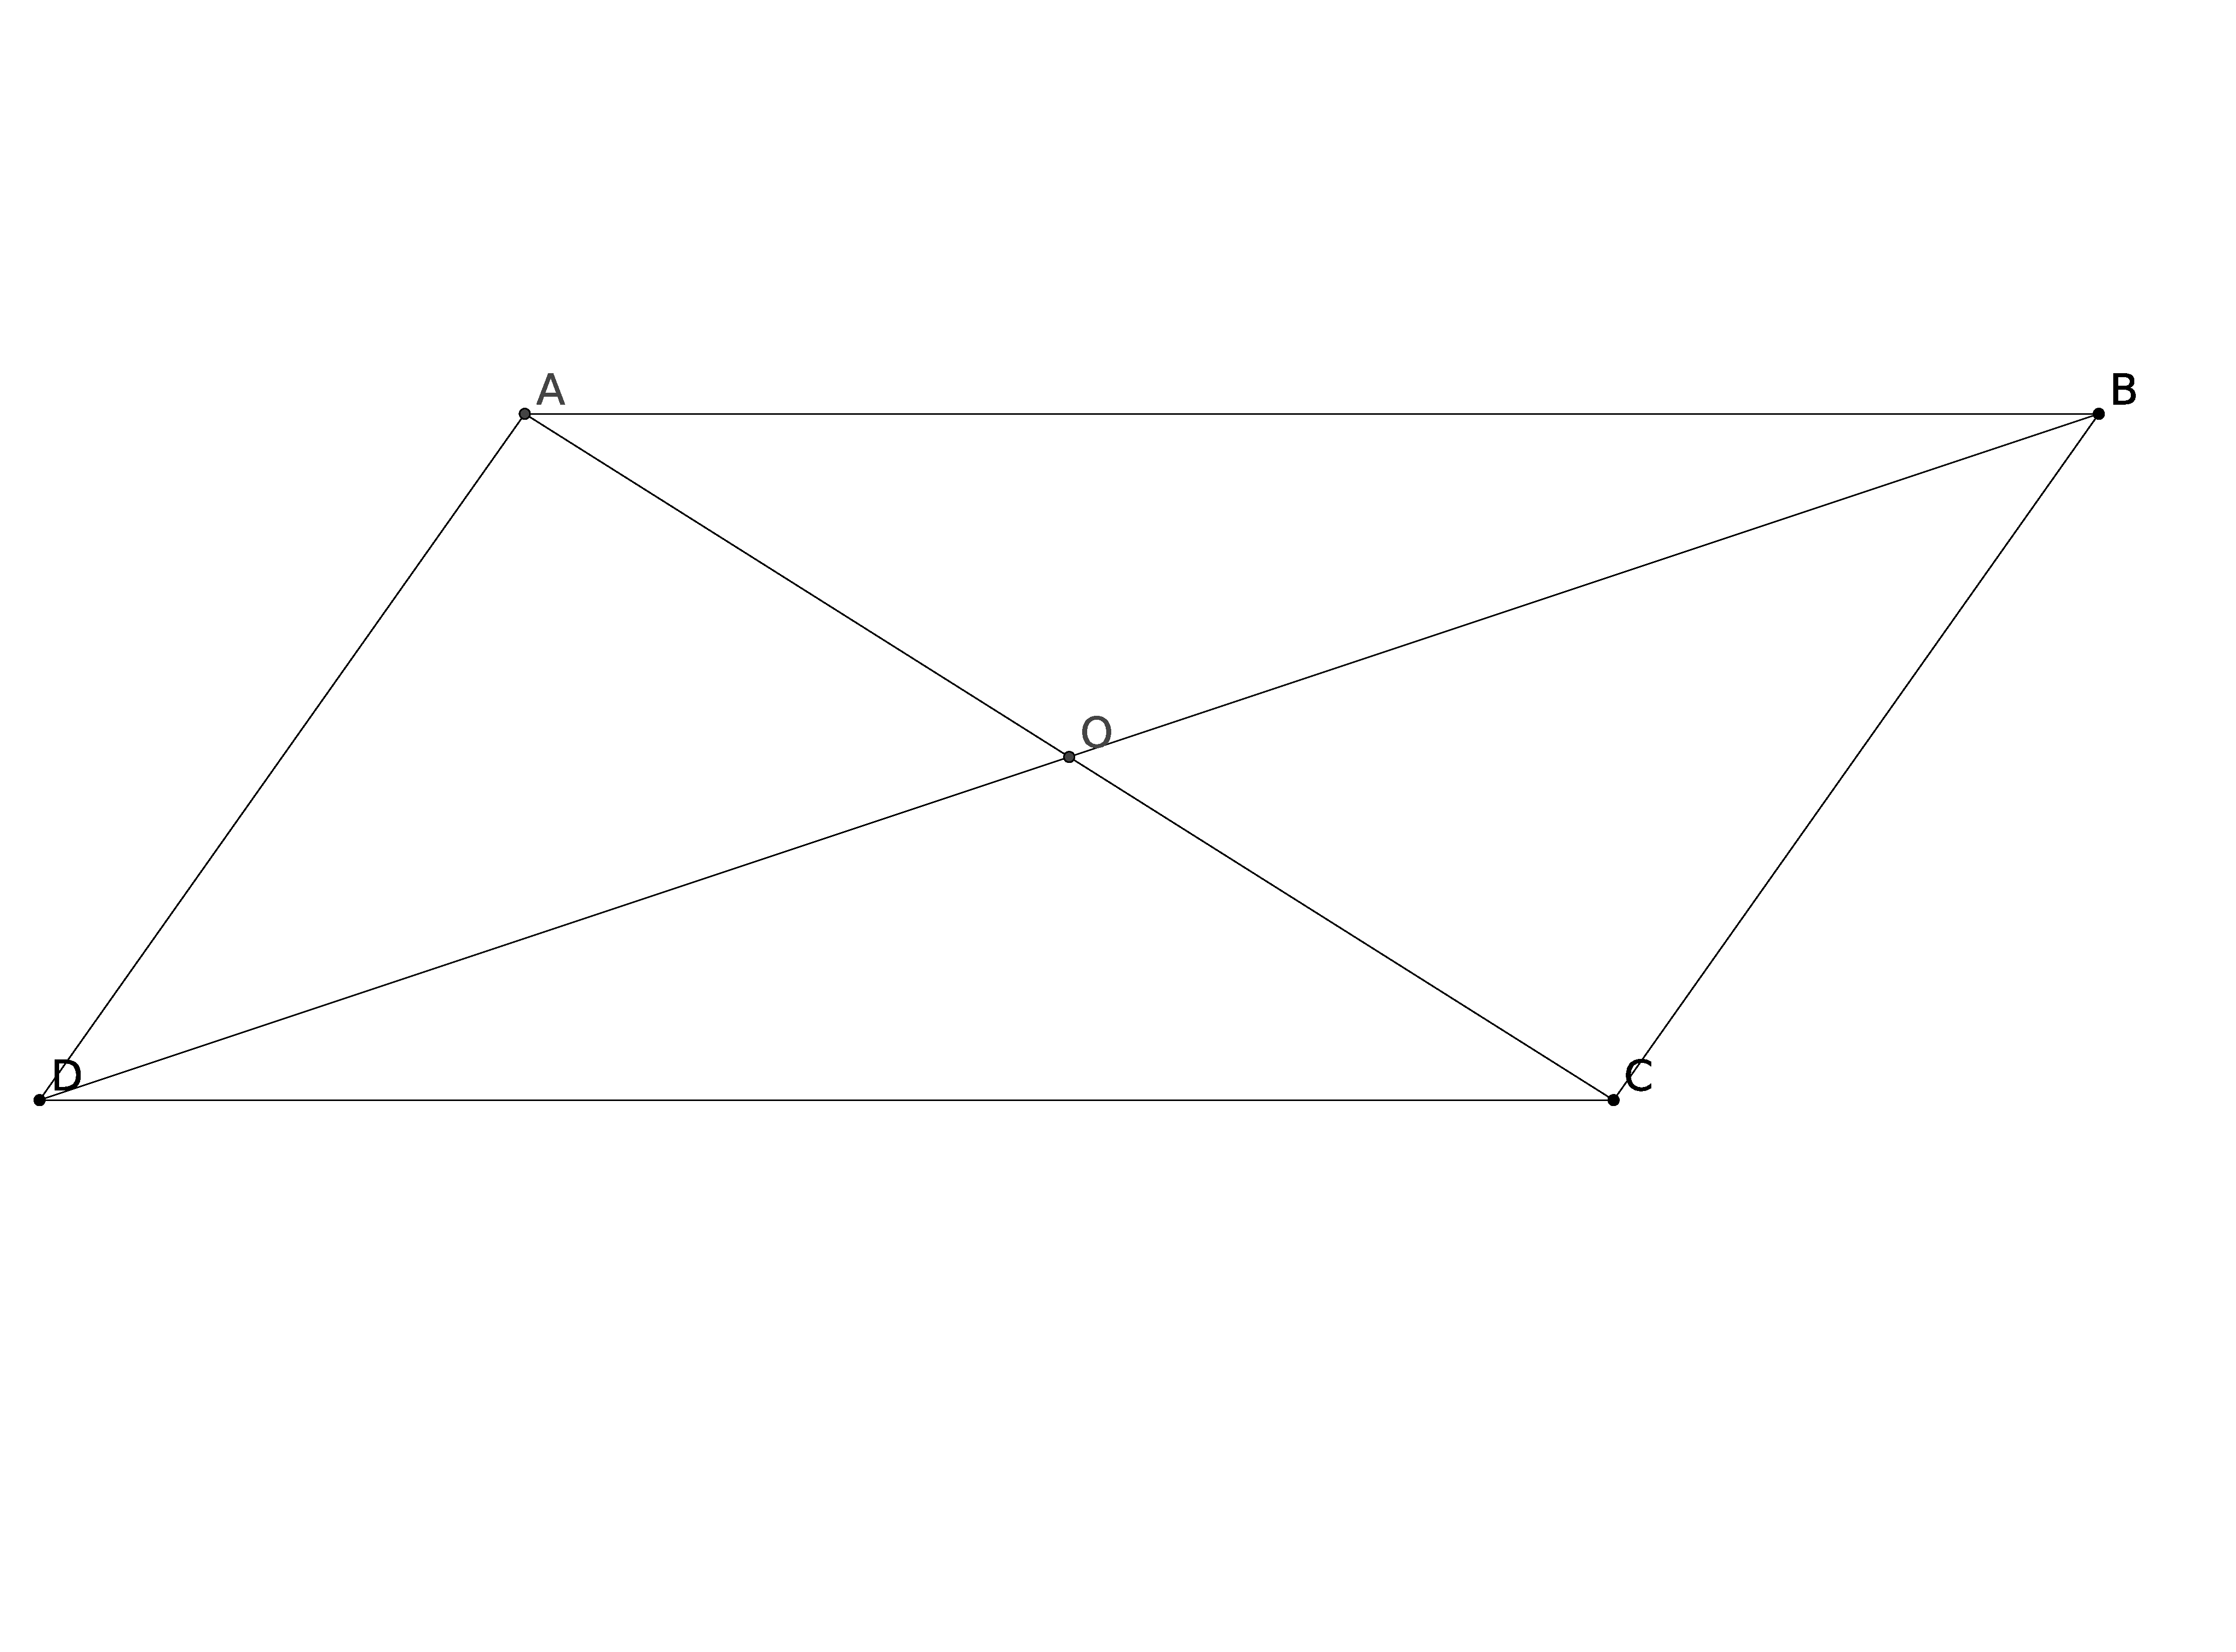
\includegraphics[scale=0.2]{parallelogram1.eps}
    \end{figure}
    
    
\begin{hyp}
$ABCD$ est un parallélogramme, donc $AB \parallel DC$ et $AD \parallel BC$.
\end{hyp}

\begin{concl}
$AO \equiv OC$, $DO \equiv OB$
\end{concl}
Puisque la définition du parallélogramme n'implique pas que les côtés opposés d'une telle figure sont isométriques, nous commençons par démontrer cela. \\
Ainsi, nous considérons les deux triangles $\triangle ABC$ et $\triangle ACD$ et nous remarquons qu'il sont isométriques grâce au théorème de la transversale (théorème \ref{th:transversale}).

\begin{figure}[H]
        \centering
        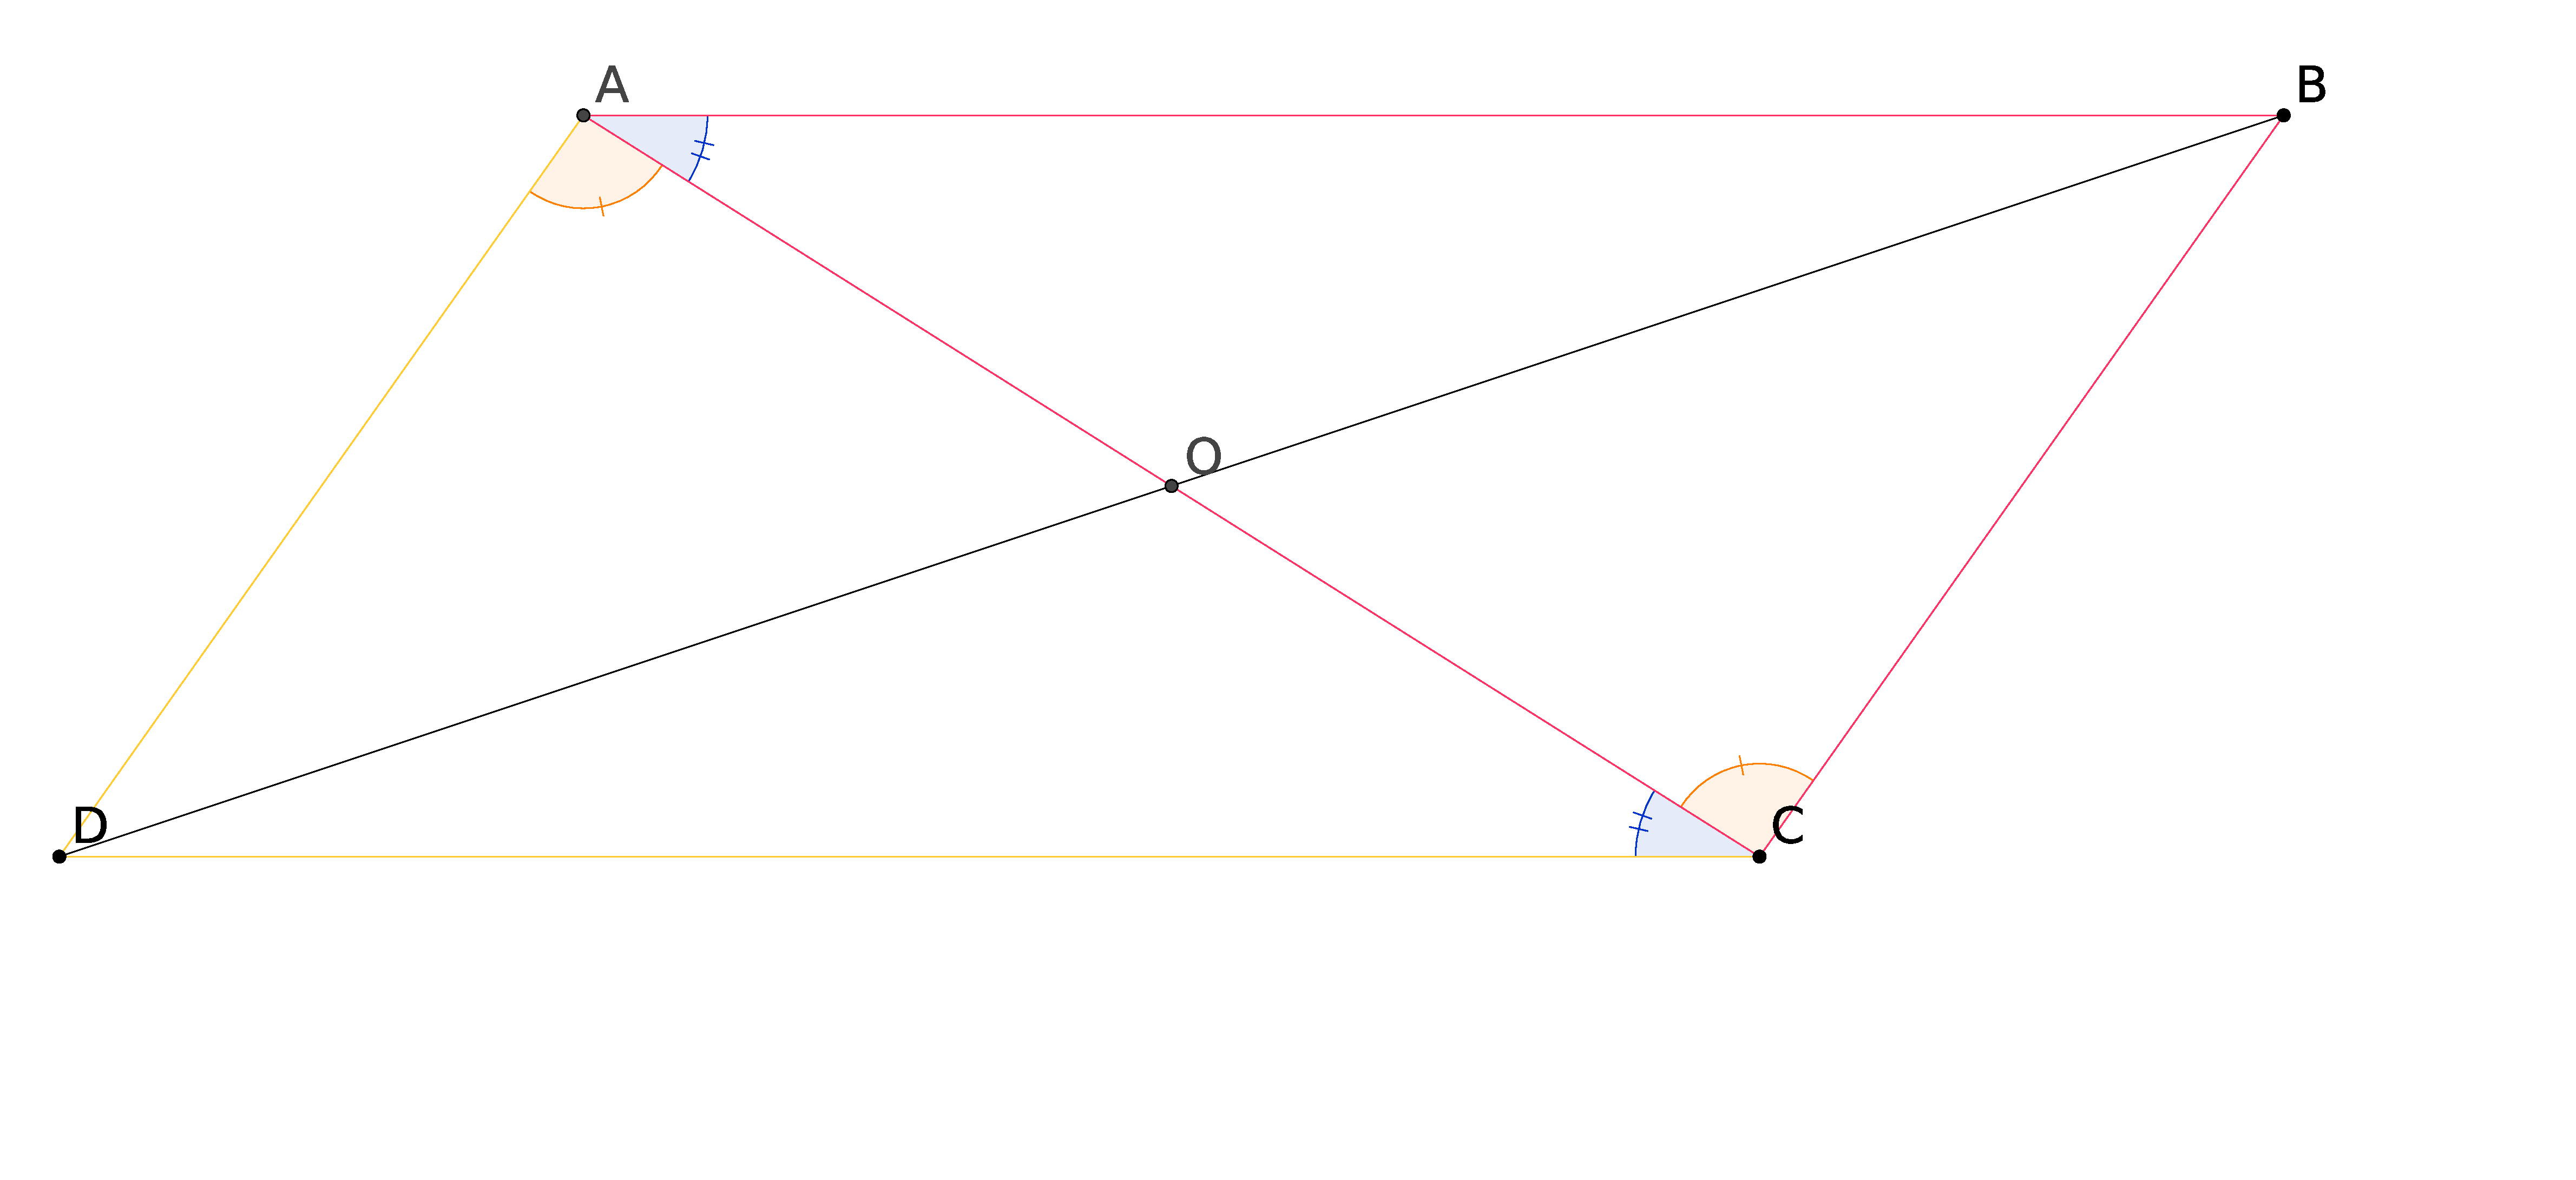
\includegraphics[scale=0.2]{parallelogram2.eps}
    \end{figure}

En effet, ces triangles respectent le deuxième cas d'isométrie des triangles, car $\angle DAC \equiv \angle ACB$, $\angle DCA \equiv \angle CAB$ et les deux triangles partagent $AC$. Nous avons donc $AB \equiv DC$ et $AD \equiv BC$.\\

A présent, grâce à l'isométrie de deux angle opposés par le sommet, on observe que que les paires d'angles $\angle AOB$/$\angle DOC$ et $\angle AOD$/$\angle COB$ sont isométriques. 

\begin{figure}[H]
        \centering
        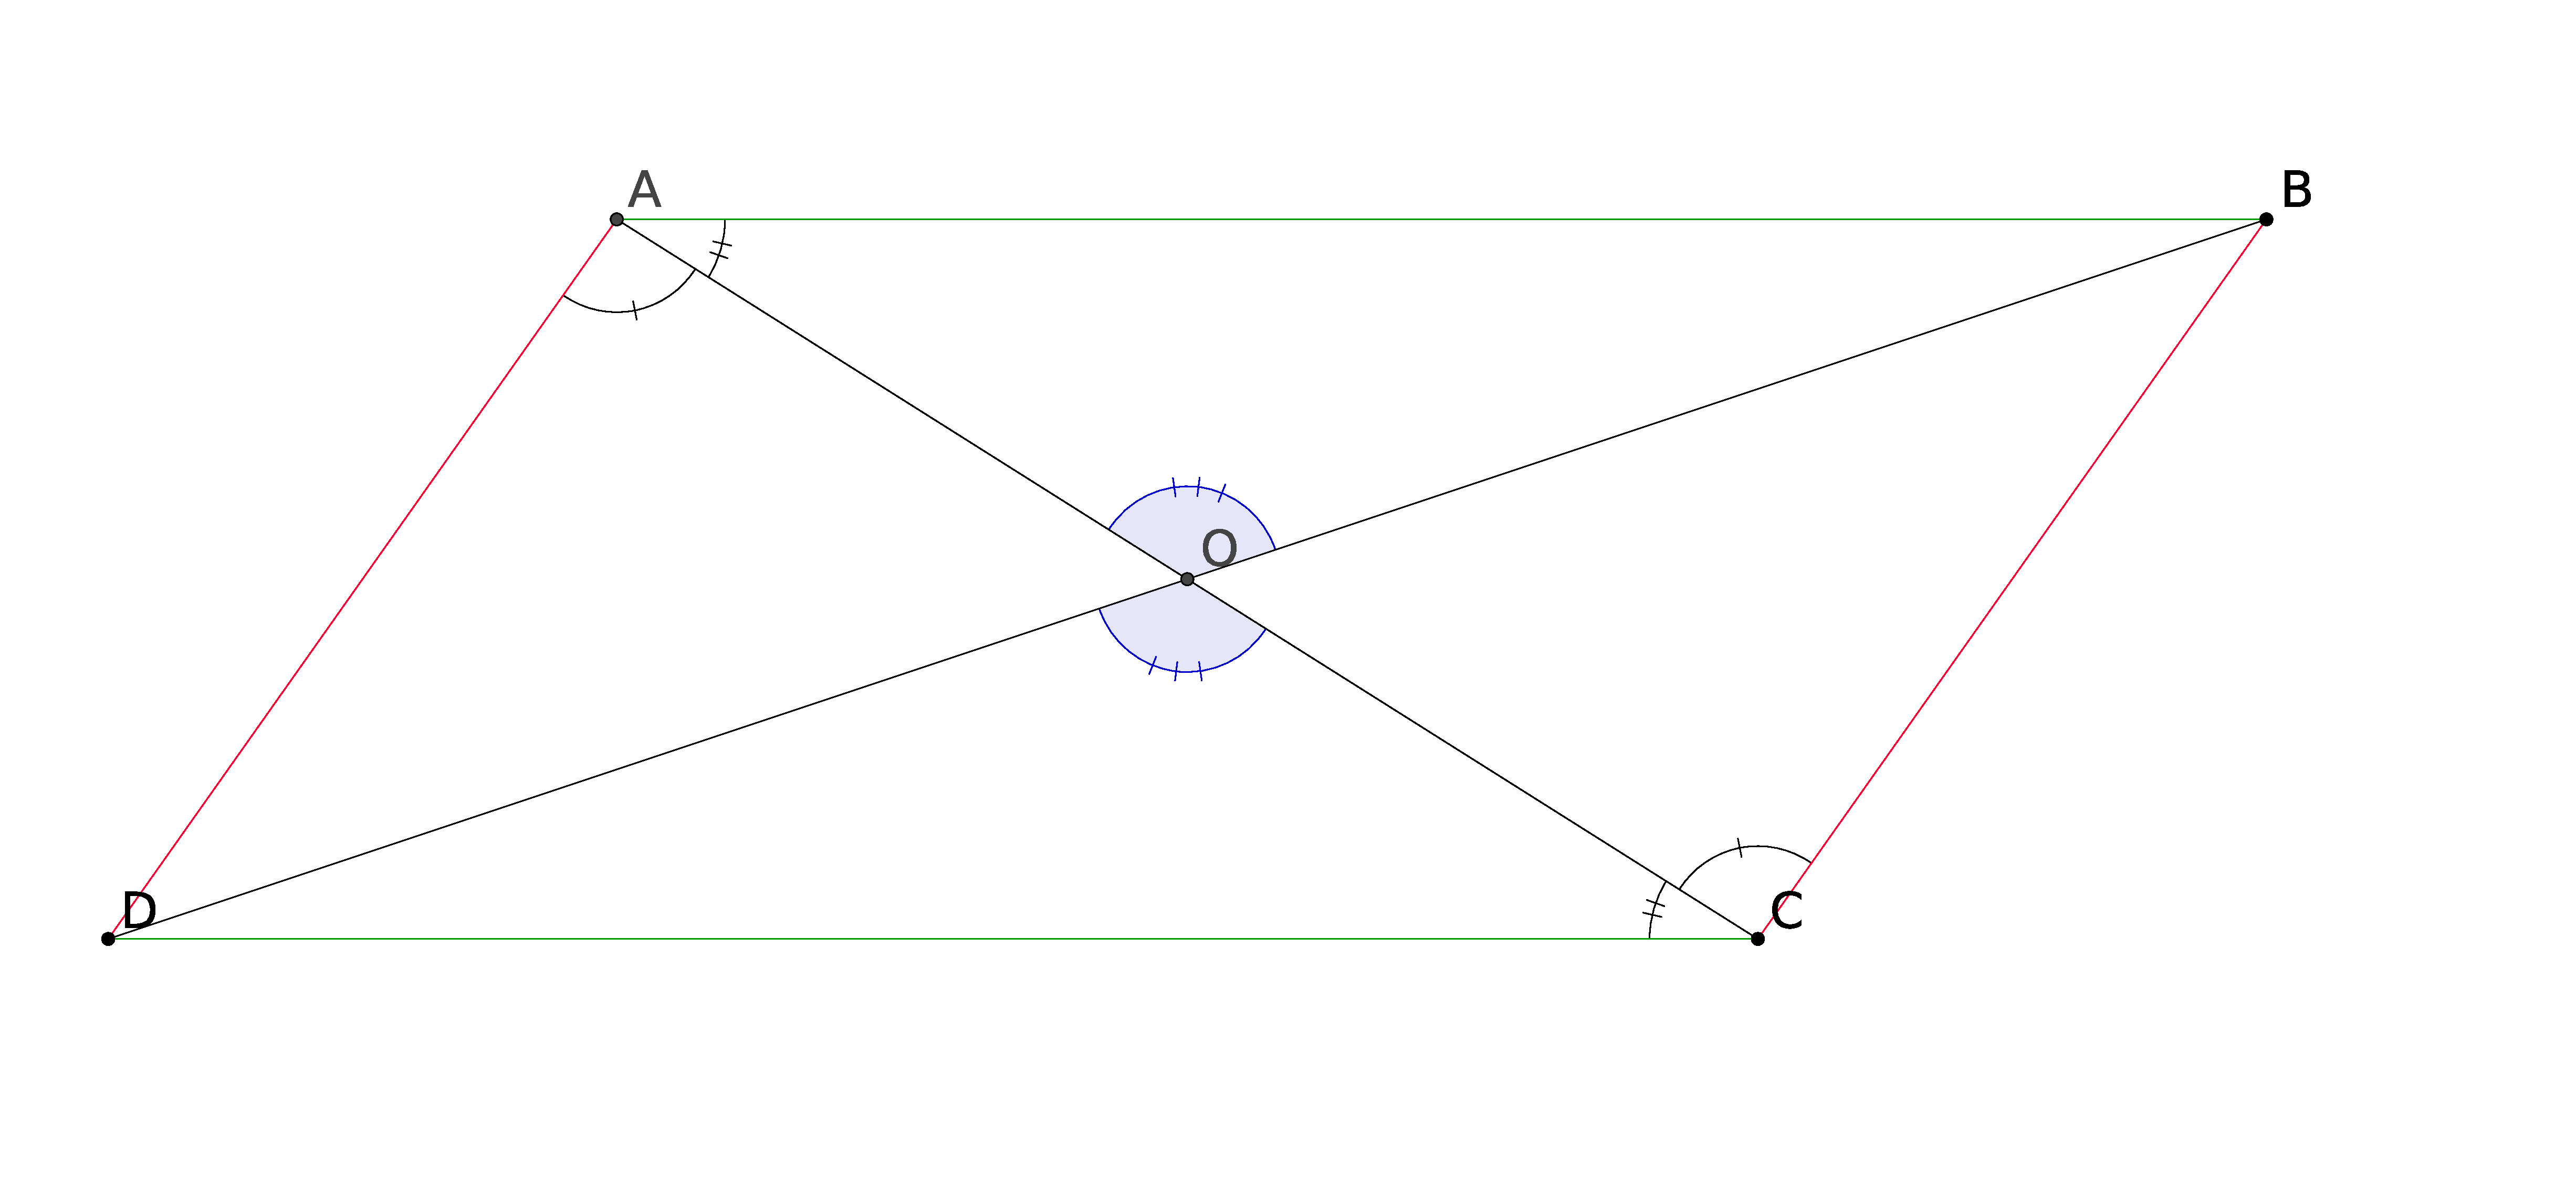
\includegraphics[scale=0.2]{parallelogram3.eps}
    \end{figure}

Par conséquent, grâce au corollaire du deuxième cas d'isométrie des triangles, les paires de triangles $\triangle AOD$/$\triangle COB$ et $\triangle AOD$/$\triangle COB$ sont isométriques. Ainsi, $AO \equiv OC$ et $DO \equiv OB$. Nous avons donc démontré que les diagonales d'un parallélogramme se coupent en leur milieu.
\end{proof}

\end{document}